\documentclass{ieeeojies}
\usepackage{cite}
\usepackage{amsmath,amssymb,amsfonts}
\usepackage{algorithmic}
\usepackage{graphicx}
\usepackage{textcomp}
\usepackage{array}
\usepackage[table]{xcolor}
\usepackage{multirow}
\usepackage{multicol}
\usepackage{float}

\def\BibTeX{{\rm B\kern-.05em{\sc i\kern-.025em b}\kern-.08em
    T\kern-.1667em\lower.7ex\hbox{E}\kern-.125emX}}

\begin{document}
\title{FORECASTING THE STOCK PRICE BY APPLYING MACHINE LEARNING AND DEEP LEARNING MODELS}

\author{\uppercase{Nguyen Thien Bao Chau}\authorrefmark{1},
\uppercase{Le Nguyen Gia Hung\authorrefmark{2}, and Nguyen Thanh Quynh Tien}\authorrefmark{3}}

\address[1]{Faculty of Information Systems, University of Information Technology, (e-mail: 21521886@gm.uit.edu.vn)}
\address[2]{Faculty of Information Systems, University of Information Technology, (e-mail: 21520890@gm.uit.edu.vn)}
\address[3]{Faculty of Information Systems, University of Information Technology, (e-mail: 21521531@gm.uit.edu.vn)}

\markboth
{Author \headeretal: Thien Bao Chau. Nguyen, Nguyen Gia Hung. Le, Thanh Quynh Tien. Nguyen}
{Author \headeretal: Thien Bao Chau. Nguyen, Nguyen Gia Hung. Le, Thanh Quynh Tien. Nguyen}

\begin{abstract}
Stock market plays an essential role in the financial field, tremendously contributing to the growth of the worldwide economy. Forecasting stock price has been the challenge mission so far due to the market’s complexity and variability. Therefore, the aim of this paper is to forecast accurately the stock price’s trend. To achieve this goal, various methods to forecast stock price such as Linear Regression (LR), Auto Regressive Integrated Moving Average (ARIMA), Support Vector Regression (SVR), Seasonal Auto Regression Integrated Moving Average (SARIMA), Dynamic Linear Model (DLM), Bagging – GRU, Simple Exponential Smoothing (SES) will be performed. The evaluation of these models using metrics such as RMSE, MAPE, and MSLE to assess model’s performance, generalization capabilities, and efficiency.
\end{abstract}

\begin{keywords}
Stock price, forecasting, ARIMA, SVR, GRU, LR, SARIMA, DLM, Bagging-GRU, SES.
\end{keywords}

\titlepgskip=-15pt

\maketitle

\section{Introduction}
\label{sec:introduction}
The stock market has been growth immensely, leading to the fact that there is the massive amount of data generated. The stock price is a complex and multifaceted problem due to the inherent uncertainty and randomness of financial markets. The motivation behind forecasting stock prices lies in the potential for generating substantial profits by accurately predicting market movements.
\\To tackle the stock prices forecasting challenge, numerous methods and techniques have been developed which ranges from statistical models to machine learning algorithms. analysis. The performed models in this paper include Linear Regression (LR), Auto Regressive Integrated Moving Average (ARIMA), Support Vector Regression (SVR), Seasonal Auto Regression Integrated Moving Average (SARIMA), Dynamic Linear Model (DLM), Bagging – GRU, Simple Exponential Smoothing (SES). These approachs provide a compresensive overview in forecasting stock price mission.
\\After developing and training these models, it is crucial to evaluate their performance and effectiveness. Various metrics can be employed to assess the models and measure their quality and capabilities. Some common metrics used for evaluation include RMSE, MAPE, and MSLE.

\section{Related Works}

In recent years, there has been a substantial amount of research dedicated to predicting stock prices using various machine learning and statistical models. \\
V. Gururaj, in a 2019 study \cite{b1}, focused on stock market prediction employing Linear Regression and Support Vector Machines, demonstrating the application of these models in forecasting stock prices.\\
Yurtsever (2021)\cite{b2} presented a study on gold price forecasting, employing LSTM, Bi-LSTM, and GRU models. The paper explores the effectiveness of these models in predicting gold prices.\\
Kishanna et al. (2022) \cite{b3} proposed a novel approach for correlation analysis, integrating FBProphet with Linear Regression to forecast market gold rates.\\
A. O. A. A. A. Ariyo (2014)\cite{b4} contributed to the literature by utilizing the ARIMA model for stock price prediction.\\
M. S. S. S. A. F. K. Senthamarai Kannan (2019)\cite{b5} compared Fuzzy Time Series and ARIMA models, providing insights into the strengths and weaknesses of these approaches.\\
B. M. Henrique et al. (2018)\cite{b6} delved into stock price prediction using Support Vector Regression on daily and up-to-the-minute prices, enhancing the understanding of SVR's applicability in different temporal contexts.\\
Gururaj also utilized exponential smoothing cells \cite{b7} , as discussed by Avner Abrami, Aleksandr Y. Aravkin, and Younghun Kim in their work from June 2017\\
Professor Thomas B. Fomby \cite{b8} made notable contributions to Exponential Smoothing Models in June 2008. \\
Eric Bauer and Ron Kohavi conducted a comprehensive comparison of voting classification algorithms, specifically focusing on Bagging, Boosting, and their variants. \cite{b9}\\
Andreas Buja and Werner Stuetzle \cite{b10} provided valuable insights into the Bagging algorithm. Buja, affiliated with the Statistics Department at The Wharton School, University of Pennsylvania, and Stuetzle from the Department of Statistics, University of Washington, Seattle, presented noteworthy observations and analyses pertaining to Bagging.\\
Henrique, Sobrero, and Kimura \cite{b11} conducted a study titled "Comparison Of Fuzzy Time Series And ARIMA." The research delves into the comparative analysis of Fuzzy Time Series and ARIMA models, exploring their effectiveness in time series forecasting. \\
Jason Brownlee \cite{b12} presented a guide on "How to Create an ARIMA Model for Time Series Forecasting in Python." The guide serves as a valuable resource for implementing ARIMA models in Python for time series forecasting.\\
Jason Brownlee \cite{b13} authored "A Gentle Introduction to SARIMA for Time Series Forecasting in Python." This work provides a user-friendly introduction to Seasonal Autoregressive Integrated Moving Average (SARIMA) models, offering insights into their application in time series forecasting. \\
Alexandra M. Schmidt and Hedibert F. Lopes \cite{b14} contributed to the field with their work on "Dynamic models." The research focuses on dynamic modeling techniques, adding valuable perspectives to the understanding of time series dynamics.\\
These works collectively contribute to the evolving landscape of stock price prediction, showcasing the versatility and effectiveness of various models across different market conditions and time frames.

\section{Materials}
\subsection{Dataset}
The historical stock price of Joint Stock Commercial Bank for Foreign Trade of Vietnam (VCB), Bank for Investment and Development of Vietnam (BIDV) and Military Commercial Joint Stock Bank (MBB) from 05/01/2016 to 27/12/2023 will be applied. The data contains column such as Date, Price, Open, High, Low, Vol., Change. As the goal is to forecast close prices, only data relating to column “Close" (VND) will be processed.

\subsection{Descriptive Statistics}
\begin{table}[H]
  \centering
  \caption{BIDV, MBB, VCB’s Descriptive Statistics}
\begin{tabular}{|>{\columncolor{red!20}}c|c|c|c|}
    \hline
     \rowcolor{red!20} & BIDV & MBB & VCB \\ \hline
     Count & 1996 & 1996 & 1996 \\ \hline
     Mean & 28,521 & 13,452 & 58,512\\ \hline
     Std & 10,778 & 6,359 & 22,722\\ \hline
     Min & 10,531 & 4,649 & 20,798\\ \hline
     25\% & 18,971 & 9,040 & 38,932\\ \hline
     50\% & 30,645 & 11,242 & 62,970\\ \hline
     75\% & 35,893 & 18,400 & 77,008\\ \hline
     Max & 49,100 & 28,667 & 106,500\\ \hline
\end{tabular}
\end{table}

\begin{figure}[H]
    \centering
    \begin{minipage}{0.23\textwidth}
    \centering
    \includegraphics[width=1\textwidth]{bibliography/Figure/BIDVboxplot.png}
    \caption{BIDV stock price's boxplot}
    \label{fig:1}
    \end{minipage}
    \hfill
    \begin{minipage}{0.23\textwidth}
    \centering
    \includegraphics[width=1\textwidth]{bibliography/Figure/BIDVhist.png}
    \caption{BIDV stock price's histogram}
    \label{fig:2}
    \end{minipage}
\end{figure}

\begin{figure}[H]
    \centering
    \begin{minipage}{0.23\textwidth}
    \centering
    \includegraphics[width=1\textwidth]{bibliography/Figure/MBboxplot.png}
    \caption{MBB stock price's boxplot}
    \label{fig:1}
    \end{minipage}
    \hfill
    \begin{minipage}{0.23\textwidth}
    \centering
    \includegraphics[width=1\textwidth]{bibliography/Figure/MBBhist.png}
    \caption{MBB stock price's histogram}
    \label{fig:2}
    \end{minipage}
\end{figure}

\begin{figure}[H]
    \centering
    \begin{minipage}{0.23\textwidth}
    \centering
    \includegraphics[width=1\textwidth]{bibliography/Figure/VCBboxplot.png}
    \caption{VCB stock price's boxplot}
    \label{fig:1}
    \end{minipage}
    \hfill
    \begin{minipage}{0.23\textwidth}
    \centering
    \includegraphics[width=1\textwidth]{bibliography/Figure/VCBhist.png}
    \caption{VCB stock price's histogram}
    \label{fig:2}
    \end{minipage}
\end{figure}

\section{Methodology}
\subsection{Linear Regression}
Regression analysis is a tool for building mathematical and statistical models that characterize relationships between a dependent variable and one or more independent, or explanatory, variables, all of which are numerical. This statistical technique is used to find an equation that best predicts the y variable as a linear function of the x variables.
A multiple linear regression model has the form: 
\[Y=\beta_0+\beta_1X_1+\beta_2X_2+\cdots+\beta_kX_k+\varepsilon\]
Where:\\
	\indent\textbullet\ Y is the dependent variable (Target Variable).\\
	\indent\textbullet\ \(X_1, X_2, \ldots, X_k\) are the independent (explanatory) variables.\\
	\indent\textbullet\ \(\beta_0\) is the intercept term.\\
	\indent\textbullet\ \(\beta_1,..., \beta_k\) are the regression coefficients for the independent variables.\\
	\indent\textbullet\ \(\varepsilon\) is the error term.
 
\subsection{Auto Regressive Integrated Moving Average (ARIMA)}
Auto Regressive Integrated Moving Average (ARIMA) is a time series forecasting cornerstone. It is a statistical method that has gained immense popularity due to its efficacy in handling various standard temporal structures in time series data. ARIMA requires a stationarity series and the component Integrated I is a method to convert the non-stationary series to a stationary series.
\\ARIMA consists of three main components:\\
\indent\textbullet\ AR (Autoregression): The autoregressive part, which models the relationship between present and past values of a time series.
\[AR(p)=\alpha+\beta_1 y_{t-1}+\beta_2 y_{t-2}+...+\beta_p y_{t-p}+\epsilon\]
\indent\textbullet\ I (Integrated): Is the process of co-integration or taking the difference.
\[I(1)=\bigtriangleup (y_t)=y_t-y_{t-1}\]
\indent\textbullet\ MA (Moving Average): Moving average, which is the process of shifting or changing the mean of a series over time.
\[MA(q)=\alpha+\theta_1 \epsilon_{t-1}+\theta_2 \epsilon_{t-2}+...+\theta_q \epsilon_{t-q}+\epsilon\]
Regression equations for ARIMA(p,d,q):
\[y_t=\beta_1 y_{t-1}+\beta_2 y_{t-2}+...+\beta_p y_{t-p}+...+\theta_1 \epsilon_{t-1}+\theta_2 \epsilon_{t-2}+\]\[...+\theta_q \epsilon_{t-q}\]
Where:\\
	\indent\textbullet\ \(y_t\) is the observed time series at time (t).\\
        \indent\textbullet\ \(\beta_1\) is the autoregressive coefficient.\\
        \indent\textbullet\ \(\phi_1\) is the moving average coefficient.\\
        \indent\textbullet\ \(\epsilon_t\)  is the white noise error term at time t.
\subsection{Support Vector Regression (SVR) }
Support Vector Regression as the name suggests is a regression algorithm that supports both linear and non-linear regressions. This method works on the principle of the Support Vector Machine. SVR differs from SVM in the way that SVM is a classifier that is used for predicting discrete categorical labels while SVR is a regressor that is used for predicting continuous ordered variables.
\\SVM kernel function:
\begin{table}[ht]
  \centering
  \caption{SVM kernel function}
\begin{tabular}{|c|c|}
    \hline
     Kernel & Function \\ \hline
     Polynomial & \(k\left(x_i,x_j\right)=\left(x_ix_j+1\right)^d\) \\ \hline
     RBF & \(K\left(x_i,y_j\right)=exp(-\gamma\|xi-xj\|^2\) \\ \hline
     Sigmoid & \(k\left(x,y\right)=tanh{\left(\alpha x^Ty+c\right)}\)\\ \hline
\end{tabular}
\end{table}
\subsection{Gated Recurrent Units (GRU)}
The GRU model is a modified version of the LSTM model, it not only merges the forget gate and the input gate into an update gate but also drops the cell state, achieved reduction of amount of parameters. A GRU unit is composed of reset gate and update gate, due to the simpler architecture, it is contributes to train faster and search optimal solution easily.
\begin{figure}[H]
    \centering
    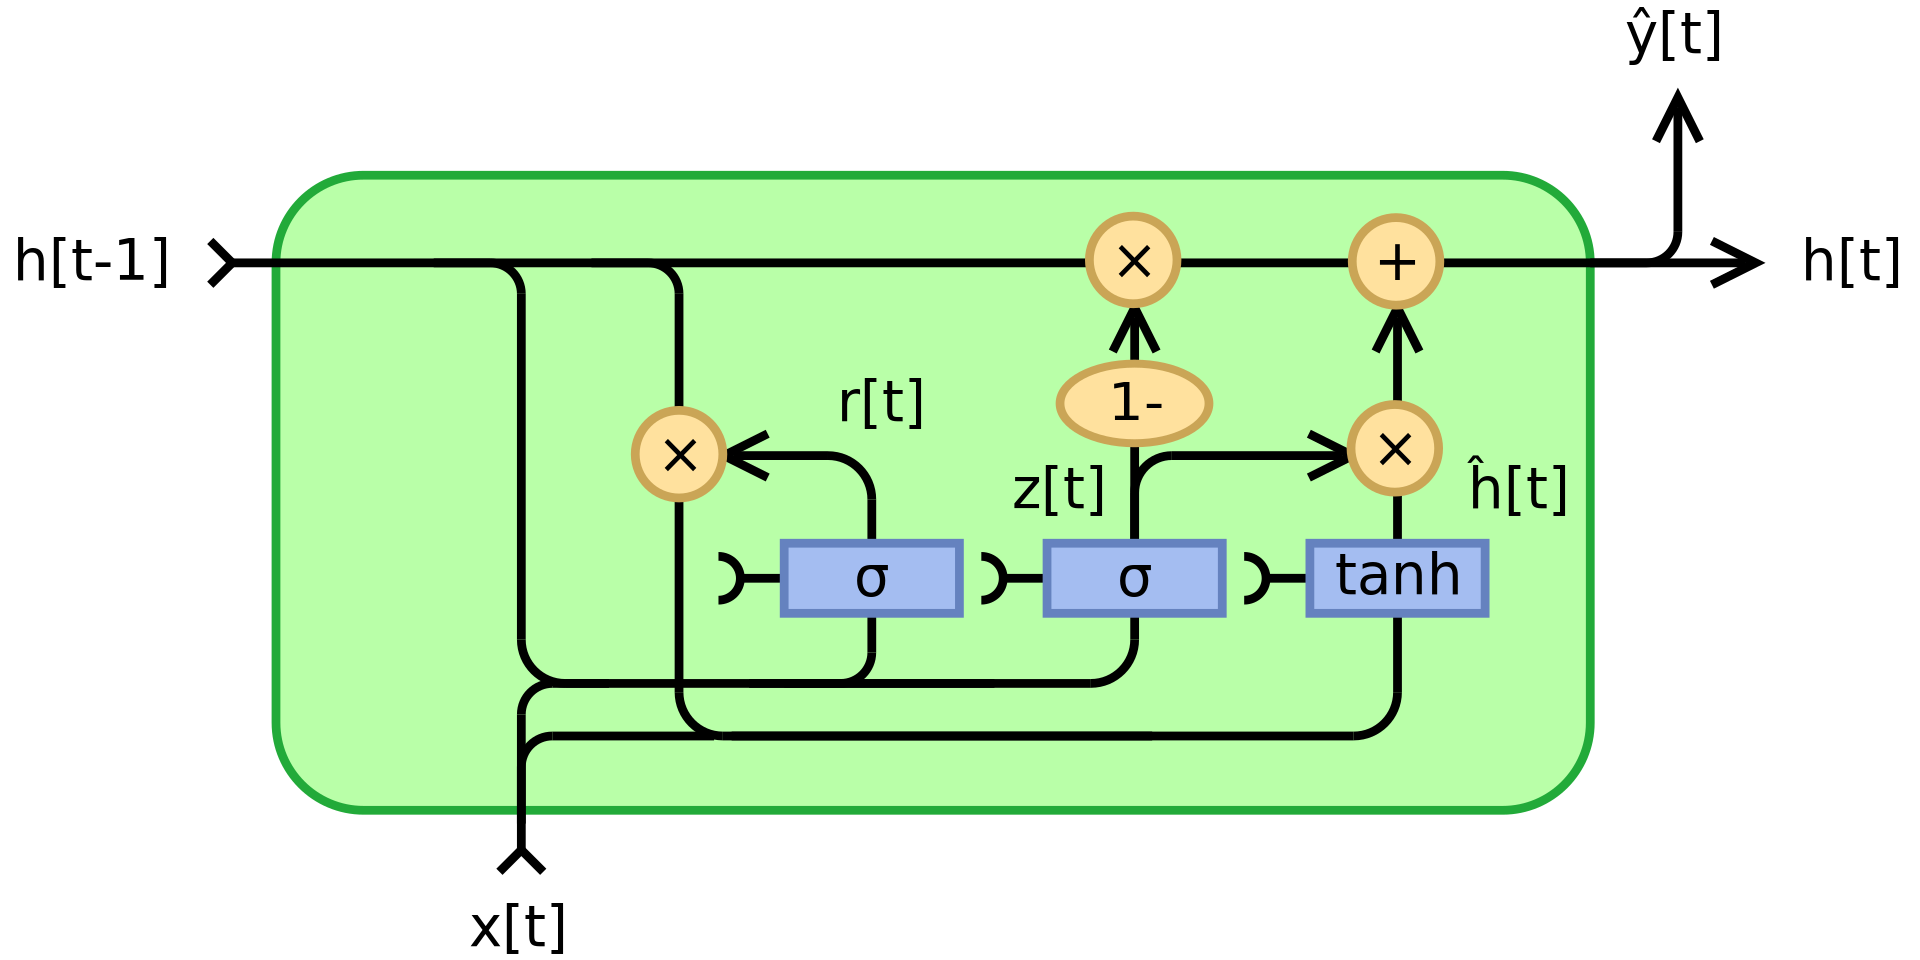
\includegraphics{bibliography/Figure/GRU.png}
    \caption{GRU model}
    \label{fig:fig7}
\end{figure}
In the first step, reset gate is calculated using both the hidden state from the previous time step and the input data at the current time step, it be reserved by applying a sigmoid function \(\sigma\), as expressed in equation:
\[r_t=\sigma{(W}_r\ast x_t+U_r\ast h_{t-1})\]
Where:\\
	\indent\textbullet\ \(x_t\) is input data at the current time step. \\
	\indent\textbullet\ \(h_{t-1}\) is the hidden state from the previous time step.\\
	\indent\textbullet\ \(W_r\) and \(U_r\) are the weighting vectors respectively.\\
Next, decided the information which will be kept from the previous time steps together with the new inputs. This equation expressed in equation:
\[{\widetilde{h}}_t=tanh{\left(W_{h^\ast}x_t+U_h\right)}\ast\left(r_{t^\ast}h_{t-1}\right)\]
Second, the update gate is computed using the previous hidden state and current input data using the same formula, like the reset gate. But each weight multiplied with the input and hidden state is independent and unique to each gate, which means the final vectors for the update gate are different from the reset gate, as expressed in equation:
\[z_t=\sigma\left(W_z\ast x_t+U_{z^\ast}h_{t-1}\right)\]
Next, summed with the output, which is from the update gate multiplied by the candidate hidden state, as expressed in equation:
\[h_t=\left(1-z_t\right)\ast h_{t-1}+z_{t^\ast}{\widetilde{h}}_t\]
\subsection{Seasonal Auto Regression Integrated Moving Average (SARIMA)}
Seasonal Autoregressive Integrated Moving Average, SARIMA or Seasonal ARIMA, is an extension of ARIMA that explicitly supports univariate time series data with a seasonal component. It adds three new hyperparameters to specify the autoregression (AR), differencing (I), and moving average (MA) for the seasonal component of the series, as well as an additional parameter for the period of the seasonality.
The model can be described in these components: SARIMA(p,d,q)(P, D, Q)s.
With:\\
\indent\textbullet\ (p,d,q) is the same as variables of ARIMA. \\
\indent\textbullet\ P: The parameter P represents the seasonal autoregressive component (the number of lags in the previous season). \\
\indent\textbullet\ D: The parameter D represents the seasonal differencing. \\
\indent\textbullet\ Q: The parameter Q represents the seasonal moving average component. \\
\indent\textbullet\ s: The parameter s denotes the length of the seasonal period in the time series.\\
The mathematical representation of SARIMA is as follows:
\[(1-\phi_1 B)(1-\Phi_1 B^s)(1-B)(1-B^s)y_t=(1+\theta_1 B)(1+\Theta_1 B^s)\epsilon_t\]
Where:\\
\indent\textbullet\ \(y_t\) is the observed time at time (t). \\
\indent\textbullet\ \(B\) is the backward shift operator, representing the lag operator (i.e.,\(By_t=y_(t-1))\)). \\
\indent\textbullet\ \(\phi_1\) is the non-seasonal autoregressive coefficient. \\
\indent\textbullet\ \(\Phi_1\) is the seasonal autoregressive coefficient. \\
\indent\textbullet\ \(\theta_1\) is the non-seasonal moving average coefficient. \\
\indent\textbullet\ \(\Theta_1\) is the seasonal moving average coefficient. \\
\indent\textbullet\ \(s\) is the seasonal period. \\
\indent\textbullet\ \(\epsilon_t\)  is the white noise error term at time (t).
\subsection{Dynamic Linear Model (DLM)}
Dynamic Linear Models (DLMs) offer a versatile approach to time series modeling, allowing for the representation of diverse temporal patterns. In contrast to traditional models like ARMA, DLMs accommodate various components such as trends, seasonality, covariates, and autoregressive elements, providing flexibility in capturing complex and non-stationary data structures. By treating time series as latent states evolving, DLMs enable the modeling of transitions influenced by dynamic components, making them suitable for tasks like short-term forecasting, intervention analysis, and monitoring. The inherent adaptability of DLMs to intricate temporal structures makes them valuable for addressing a wide range of real-world applications.
\\The following observation and evolution equations define a Dynamic Linear Model:\\
\indent\textbullet\ Observation Equation:
\[y_t=F_t^T \theta_t+\epsilon_t,\epsilon_t~N[0,V_t]\]
\indent\textbullet\ Evolution Equation:
\[\theta_t=G_t \theta_{t+1}+\omega_t,\omega_t~N[0,W_t]\]

\subsection{Bagging - GRU}
Bagging, also referred to as Bootstrap aggregating, is an ensemble learning method that enhances the performance and accuracy of machine learning algorithms. It addresses the trade-off between bias and variance, effectively reducing the variability in prediction models. GRU is a machine learning model which is mentioned above.
\begin{figure}[H]
    \centering
    \includegraphics[width=0.4\textwidth]{bibliography/bagging.png}
    \caption{Bagging algorithm}
    \label{fig:bagging}
\end{figure}
When applying bagging to a GRU model, the goal is to create an ensemble of GRU models that work together to make predictions.

\subsection{Simple Exponential Smoothing (SES)}
Exponential smoothing methods model current and future time series observations as a weighted combinations of past observations, with more weight given to recent data. The word ‘exponential’ reflects the exponential decay of weights for older observations. Exponential smoothing provides simple and interpretable models and forecasting capability by assuming a fixed structure for the evolution of the time series.\\
A Simple Exponential Smoothing model is:
\[\hat{y}_{t+1} = \hat{y}_t + \alpha(y_t - \hat{y}_t) = (1 - \alpha)\hat{y}_t + \alpha y_t\]
Where:\\
    \indent\textbullet\ \(y_t\) is the observed value at time t. \\
    \indent\textbullet\ \(\hat{y}_t\) is the predicted value at time t. \\
    \indent\textbullet\ \(\alpha\) is the smoothing parameter.


\section{Result}
\subsection{Evaluation Methods}
\textbf{Mean Percentage Absolute Error} (MAPE): is the average percentage error in a set of predicted values.\\
\[MAPE=\frac{100\%}{n}  \sum_{i=1}^{n} |y_i-\hat{y_i} |  = 1 \]\\
\textbf{Root Mean Squared Error} (RMSE): is the square root of average value of squared error in a set of predicted values.\\
\[RMSE=\sqrt{\sum_{i=1}^{n} \frac{(\hat{y_i}-y_i )^2}{n} }\]\\
\textbf{Mean Absolute Error} (MSLE):is the relative difference between the log-transformed actual and predicted values.\\
\[MSLE=\frac{1}{n}\sum_{i=1}^{n}(log(1+\hat{y_i})-log(log(1+y_i))^2\]
Where: \\
	\indent\textbullet\ \(n\) is the number of observations in the dataset.\\
	\indent\textbullet\ \(y_i\)  is the true value.\\
	\indent\textbullet\ \(\hat{y_i}\) is the predicted value.
\subsection{VCB Dataset} 
\begin{table}[H]
    \centering
    \begin{tabular}{|c|c|c|c|c|}
         \hline
         \multicolumn{5}{|c|}{\textbf{VCB Dataset's Evaluation}}\\
         \hline
         \centering Model & Training:Testing & RMSE & MAPE (\%) & MSLE\\
         \hline
         \multirow{2}{*}{LN} & 7:3 & 10508.77 & 10.71 & 0.015 \\ & 8:2 & 11729.2 & 10.825 & 0.019 \\ & \textbf{9:1} & \textbf{7933.49} & \textbf{7.47} & \textbf{0.007}\\
         \hline
         \multirow{2}{*}{SVR} & 7:3&11864.3&7.52&0.021\\ & 8:2&8521.33&5.01&0.009 \\ & \textbf{9:1} & \textbf{7006.54} & \textbf{3.73} & \textbf{0.006}\\
         \hline
         \multirow{2}{*}{GRU} & \textbf{7:3}	& \textbf{1545.676} & \textbf{1.262} & \textbf{0.00033} \\ & 8:2 & 1616.817 & 1.267 & 0.00035 \\ & 9:1 & 1699.655  & 1.052 & 0.00032\\
         \hline
         \multirow{2}{*}{ARIMA} & 7:3 &  8620.284 &  8.559 & 0.01 \\ & 8:2 &  11729.2 & 10.825 & 0.019 \\ & \textbf{9:1} & \textbf{7644.773}  & \textbf{7.287} & \textbf{0.007}\\
         \hline
         \multirow{2}{*}{SARIMA} & \textbf{7:3}	& \textbf{7971.644} & \textbf{7.755} & \textbf{0.009} \\ & 8:2 & 11711.484 & 10.809 & 0.019 \\ & 9:1 & 8629.708 & 8.253 & 0.009\\
         \hline
         \multirow{2}{*}{DLM} & 7:3 & 13156.831&13.336 & 0.021 \\ & \textbf{8:2} &	\textbf{7209.84} & \textbf{7.093} & \textbf{0.007} \\ & 9:1 &11945.338	&11.444&0.016\\
         \hline
         \multirow{2}{*}{SES} & 7:3 & 10949.0750 & 9.4738 & 0.0169 \\ & 8:2 & 11717.8586 &10.8142 & 0.0189 \\ & \textbf{9:1} &  	\textbf{6000.7953} &	\textbf{5.2412} & 	\textbf{0.004} \\
         \hline
         \multirow{2}{*}{BaggingGRU} & 7:3 & 941.7588 &  1.7384 &  0.0005 \\ & 8:2 & 939.7588 &  1.6546 &  0.0005 \\ & \textbf{9:1} & \textbf{936.8374} & \textbf{1.6273} & \textbf{0.0005}\\
         \hline
    \end{tabular}
    \caption{VCB Dataset's Evaluation}
    \label{vcbresult}
\end{table}

\begin{figure}[H]
  \centering
  \begin{minipage}{0.8\linewidth}
    \centering
    \includegraphics[width=\linewidth]{bibliography/LN_VCB91.png}
    \caption{Linear model's result with 9:1 splitting proportion}
    \label{fig8}
  \end{minipage}
\end{figure}
\begin{figure}[H]
  \centering
  \begin{minipage}{0.8\linewidth}
    \centering
    \includegraphics[width=\linewidth]{bibliography/SVR_VCB91.png}
    \caption{SVR model's result with 9:1 splitting proportion}
    \label{fig9}
  \end{minipage}
\end{figure}
\begin{figure}[H]
  \centering
  \begin{minipage}{0.8\linewidth}
    \centering
    \includegraphics[width=\linewidth]{bibliography/GRU_VCB73.png}
    \caption{GRU model's result with 7:3 splitting proportion}
    \label{fig10}
  \end{minipage}
\end{figure}
\begin{figure}[H]
  \centering
  \begin{minipage}{0.8\linewidth}
    \centering
    \includegraphics[width=\linewidth]{bibliography/ARIMA_VCB91.png}
    \caption{ARIMA model's result with 9:1 splitting proportion}
    \label{fig11}
  \end{minipage}
\end{figure}
\begin{figure}[H]
  \centering
  \begin{minipage}{0.8\linewidth}
    \centering
    \includegraphics[width=\linewidth]{bibliography/SARIMA_VCB73.png}
    \caption{SARIMA model's result with 7:3 splitting proportion}
    \label{fig12}
  \end{minipage}
\end{figure}
\begin{figure}[H]
  \centering
  \begin{minipage}{0.8\linewidth}
    \centering
    \includegraphics[width=\linewidth]{bibliography/DLM_VCB82.png}
    \caption{DLM model's result with 8:2 splitting proportion}
    \label{fig13}
  \end{minipage}
\end{figure}
\begin{figure}[H]
  \centering
  \begin{minipage}{0.8\linewidth}
    \centering
    \includegraphics[width=\linewidth]{bibliography/ETS_VCB91.png}
    \caption{SES model's result with 9:1 splitting proportion}
    \label{fig14}
  \end{minipage}
\end{figure}
\begin{figure}[H]
  \centering
  \begin{minipage}{0.8\linewidth}
    \centering
    \includegraphics[width=\linewidth]{bibliography/baggingGRU_vcb.png}
    \caption{Bagging-GRU model's result with 8:2 splitting proportion}
    \label{bagginggru}
  \end{minipage}
\end{figure}
\subsection{MBB dataset} 
\begin{table}[H]
    \centering
    \begin{tabular}{|c|c|c|c|c|}
         \hline
         \multicolumn{5}{|c|}{\textbf{MBB Dataset's Evaluation}}\\
         \hline
         \centering Model & Training:Testing & RMSE & MAPE (\%) & MSLE\\
         \hline
         \multirow{2}{*}{LN} & \textbf{7:3}&\textbf{4983.47}&\textbf{17.44}&\textbf{0.058} \\ & 8:2 &  5293.6 & 26.28 & 0.063 \\ & 9:1&4894.46&25.85&0.055\\
         \hline
         \multirow{2}{*}{SVR} & 7:3&977.55&1.76&0.002 \\ & 8:2&242.75&0.89&0.0002 \\ & \textbf{9:1} & \textbf{162.85} & \textbf{0.75} & \textbf{0.00008}\\
         \hline
         \multirow{2}{*}{GRU} & 7:3&454.9923&1.54&0.0005 \\ &  8:2&388.5658&1.406&	0.0005 \\ & \textbf{9:1} & \textbf{373.744} & \textbf{1.36} & \textbf{0.00038}\\
         \hline
         \multirow{2}{*}{ARIMA} & 7:3 & 9682.514 & 43.586 & 0.161 \\ & 8:2 & 7136.268 & 36.166 & 0.106 \\ & \textbf{9:1} & \textbf{1139.476} & \textbf{4.57} & \textbf{0.004}\\
         \hline
         \multirow{2}{*}{SARIMA} & 7:3 & 9693.439 & 43.648&0.162 \\ &8:2 & 4564.211 & 23.154 & 0.05 \\ &  \textbf{9:1} &  \textbf{1137.416} &  \textbf{4.564} &  \textbf{0.004}\\
         \hline
         \multirow{2}{*}{DLM} & 7:3 & 9428.531 & 41.483 & 0.154 \\ & 8:2 & 7054.485 & 34.819 & 0.102\\ & \textbf{9:1} & \textbf{1297.301} & \textbf{5.744} & \textbf{0.005}\\
         \hline
         \multirow{2}{*}{SES} & 7:3 &  4988.1456 & 22.7511 & 0.0546 \\ & 8:2 & 4659.5801 & 23.6876 & 0.0516 \\ & \textbf{9:1} &  \textbf{1137.4155} &	\textbf{4.5635} & 	\textbf{0.0036} \\
         \hline
         \multirow{2}{*}{BaggingGRU} & 7:3 & 941.7588 &  1.7384 &  0.0005 \\ & 8:2 & 939.7588 &  1.6546 &  0.0005 \\ & \textbf{9:1} & \textbf{936.8374} & \textbf{1.6273} & \textbf{0.0005}\\
         \hline
    \end{tabular}
    \caption{MBB Dataset's Evaluation}
    \label{mbbresult}
\end{table}

\begin{figure}[H]
  \centering
  \begin{minipage}{0.8\linewidth}
    \centering
    \includegraphics[width=\linewidth]{bibliography/LN_MBB73.png}
    \caption{Linear model's result with 7:3 splitting proportion}
    \label{fig15}
  \end{minipage}
\end{figure}
\begin{figure}[H]
  \centering
  \begin{minipage}{0.8\linewidth}
    \centering
    \includegraphics[width=\linewidth]{bibliography/SVR_MBB91.png}
    \caption{SVR model's result with 9:1 splitting proportion}
    \label{fig16}
  \end{minipage}
\end{figure}
\begin{figure}[H]
  \centering
  \begin{minipage}{0.8\linewidth}
    \centering
    \includegraphics[width=\linewidth]{bibliography/GRU_MBB91.png}
    \caption{GRU model's result with 9:1 splitting proportion}
    \label{fig17}
  \end{minipage}
\end{figure}
\begin{figure}[H]
  \centering
  \begin{minipage}{0.8\linewidth}
    \centering
    \includegraphics[width=\linewidth]{bibliography/ARIMA_MBB91.png}
    \caption{ARIMA model's result with 9:1 splitting proportion}
    \label{fig18}
  \end{minipage}
\end{figure}
\begin{figure}[H]
  \centering
  \begin{minipage}{0.8\linewidth}
    \centering
    \includegraphics[width=\linewidth]{bibliography/SARIMA_MBB91.png}
    \caption{SARIMA model's result with 9:1 splitting proportion}
    \label{fig19}
  \end{minipage}
\end{figure}
\begin{figure}[H]
  \centering
  \begin{minipage}{0.8\linewidth}
    \centering
    \includegraphics[width=\linewidth]{bibliography/DLM_MBB91.png}
    \caption{DLM model's result with 9:1 splitting proportion}
    \label{fig20}
  \end{minipage}
\end{figure}
\begin{figure}[H]
  \centering
  \begin{minipage}{0.8\linewidth}
    \centering
    \includegraphics[width=\linewidth]{bibliography/ETS_MBB91.png}
    \caption{SES model's result with 9:1 splitting proportion}
    \label{fig21}
  \end{minipage}
\end{figure}
\begin{figure}[H]
  \centering
  \begin{minipage}{0.8\linewidth}
    \centering
    \includegraphics[width=\linewidth]{bibliography/baggingGRU_MBB.png}
    \caption{Bagging-GRU model's result with 9:1 splitting proportion}
    \label{mbbbggg}
  \end{minipage}
\end{figure}
\subsection{BIDV dataset} 
\begin{table}[H]
    \centering
    \begin{tabular}{|c|c|c|c|c|}
         \hline
         \multicolumn{5}{|c|}{\textbf{Dataset's Evaluation}}\\
         \hline
         \centering Model & Training:Testing & RMSE & MAPE (\%) & MSLE\\
         \hline
         \multirow{2}{*}{LN} & 7:3 & 5690.9 & 13.03 & 0.021 \\ & 8:2 & 4904.44 & 10.28 & 0.016 \\ & \textbf{9:1} & \textbf{2859.97} & \textbf{5.49} & \textbf{0.004} \\
         \hline
         \multirow{2}{*}{SVR} & 7:3 & 5212.21 & 7.55 & 0.016 \\ & 8:2 & 1014.97 & 1.62 & 0.0005 \\ & \textbf{9:1} & \textbf{822.63} & \textbf{1.26} & \textbf{0.0003}\\
         \hline
         \multirow{2}{*}{GRU} & 7:3 & 916.692 & 1.67 & 0.00055 \\ &  8:2 & 948.341 & 1.74 & 0.00057 \\ & \textbf{9:1} &. \textbf{761.754} & \textbf{1.21} & \textbf{0.0003}\\
         \hline
         \multirow{2}{*}{ARIMA} & 7:3 & 7847.594 & 15.278 & 0.041 \\ & 8:2 & 7501.223 & 15.14 & 0.036 \\ & \textbf{9:1} & \textbf{3371.058} & \textbf{6.414} & \textbf{0.006}\\
         \hline
         \multirow{2}{*}{SARIMA} & 7:3 & 7849.75 & 15.29 & 0.04 \\ &8:2 &7501.73 & 15.15 & 0.04 \\ &  \textbf{9:1} & \textbf{3373.34} & \textbf{6.43} & \textbf{0.006}\\
         \hline
         \multirow{2}{*}{DLM} & 7:3 & 4288.68 & 8.641 & 0.012\\ & 8:2 & 3771.703	& 7.756 & 0.009\\ & \textbf{9:1} & \textbf{3617.388} & \textbf{6.446} & \textbf{0.007}\\
         \hline
         \multirow{2}{*}{SES} & 7:3 &  7849.6833 & 15.2872 & 0.0407 \\ & 8:2 & 7502.4992 & 15.1483 & 0.0357 \\ & \textbf{9:1} &  \textbf{3342.8102} &	\textbf{6.3561} & 	\textbf{0.0057} \\
         \hline
         \multirow{2}{*}{BaggingGRU} & 7:3 & 941.7588 &  1.7384 &  0.0005 \\ & 8:2 & 939.7588 &  1.6546 &  0.0005 \\ & \textbf{9:1} & \textbf{936.8374} & \textbf{1.6273} & \textbf{0.0005}\\
         \hline
    \end{tabular}
    \caption{BIDV Dataset's Evaluation}
    \label{mbbresult}
\end{table}

\begin{figure}[H]
  \centering
  \begin{minipage}{0.8\linewidth}
    \centering
    \includegraphics[width=\linewidth]{bibliography/LN_BIDV91.png}
    \caption{Linear model's result with 9:1 splitting proportion}
    \label{fig22}
  \end{minipage}
\end{figure}
\begin{figure}[H]
  \centering
  \begin{minipage}{0.8\linewidth}
    \centering
    \includegraphics[width=\linewidth]{bibliography/SVR_BIDV91.png}
    \caption{SVR model's result with 9:1 splitting proportion}
    \label{fig23}
  \end{minipage}
\end{figure}
\begin{figure}[H]
  \centering
  \begin{minipage}{0.8\linewidth}
    \centering
    \includegraphics[width=\linewidth]{bibliography/GRU_BIDV91.png}
    \caption{GRU model's result with 9:1 splitting proportion}
    \label{fig24}
  \end{minipage}
\end{figure}
\begin{figure}[H]
  \centering
  \begin{minipage}{0.8\linewidth}
    \centering
    \includegraphics[width=\linewidth]{bibliography/ARIMA_BIDV91.png}
    \caption{ARIMA model's result with 9:1 splitting proportion}
    \label{fig25}
  \end{minipage}
\end{figure}
\begin{figure}[H]
  \centering
  \begin{minipage}{0.8\linewidth}
    \centering
    \includegraphics[width=\linewidth]{bibliography/SARIMA_BIDV91.png}
    \caption{SARIMA model's result with 9:1 splitting proportion}
    \label{fig26}
  \end{minipage}
\end{figure}
\begin{figure}[H]
  \centering
  \begin{minipage}{0.8\linewidth}
    \centering
        \includegraphics[width=\linewidth]{bibliography/BIDV_DLM91.png}
    \caption{DLM model's result with 9:1 splitting proportion}
    \label{fig27}
  \end{minipage}
\end{figure}
\begin{figure}[H]
  \centering
  \begin{minipage}{0.8\linewidth}
    \centering
        \includegraphics[width=\linewidth]{bibliography/ETS_BIDV91.png}
    \caption{SES model's result with 9:1 splitting proportion}
    \label{fig28}
  \end{minipage}
\end{figure}
\begin{figure}[H]
  \centering
  \begin{minipage}{0.8\linewidth}
    \centering
        \includegraphics[width=\linewidth]{bibliography/baggingGRU_BIDV.png}
    \caption{Bagging-GRU model's result with 7:3 splitting proportion}
    \label{fig28}
  \end{minipage}
\end{figure}
\section{Conclusion}
\subsection{Summary}
In the achievement of forecasting stock prices, the exploration of diverse methodologies, ranging from traditional statistical models to advanced machine learning algorithms, has been aimed. Among the performed models, Linear Regression (LR), Auto Regressive Integrated Moving Average (ARIMA), Support Vector Regression (SVR), Seasonal Auto Regression Integrated Moving Average (SARIMA), Dynamic Linear Model (DLM), Bagging – GRU, and Simple Exponential Smoothing (SES), it becomes evident that Support Vector Regression (SVR), Gated Recurrent Unit (GRU), and Bagging GRU emerge as the most promising and effective models for predicting stock prices.\\
The intricacies of stock price forecasting, rooted in the complexity and unpredictability of financial markets, demand models that can capture nuanced patterns and relationships within the data. Support Vector Regression (SVR) showcases its efficacy in handling intricate relationships, providing robust predictions. Gated Recurrent Unit (GRU) models, with their ability to capture sequential dependencies, exhibit notable performance in forecasting stock prices. The introduction of ensemble learning through Bagging GRU further refines the predictive capabilities, offering a collective insight that surpasses individual models.\\
As evidenced by the evaluation metrics, including RMSE, MAPE, and MSLE, the SVR, GRU, and Bagging GRU models consistently demonstrate superior performance across various aspects of forecasting accuracy. Their adaptability to handle the inherent uncertainties of stock markets positions them as formidable tools for investors and analysts seeking reliable predictions.
\subsection{Future Considerations}
In our future research, it is crucial to prioritize further optimization of the previously mentioned models. This optimization effort should specifically focus on:\\
\indent\textbullet\ Enhancing the accuracy of the model. While the above algorithms have demonstrated promising results in predicting stock prices, there is a need to further improve the model's accuracy to ensure more precise forecasting outcomes.\\
\indent\textbullet\ Exploring alternative machine learning algorithms or ensemble techniques. Ensemble techniques, such as combining multiple models or using various ensemble learning methods, can also improve the robustness and accuracy of the forecasts.\\
\indent\textbullet\ Researching new forecasting models. The field of forecasting continuously evolves, with new algorithms and models being researched and developed. It is crucial to stay updated with these approaches and explore new forecasting models that offer improved accuracy and performance. \\
By continuously exploring and incorporating new features, data sources, and modeling techniques, we can strive for ongoing optimization of the forecasting models and enhance their ability to predict stock prices with greater precision and reliability.
\section*{Acknowledgment}
\addcontentsline{toc}{section}{Acknowledgment}
First and foremost, we would like to express our sincere gratitude to \textbf{Assoc. Prof. Dr. Nguyen Dinh Thuan} and \textbf{Mr. Nguyen Minh Nhut} for their exceptional guidance, expertise, and invaluable feedback throughout the research process. Their mentorship and unwavering support have been instrumental in shaping the direction and quality of this study. Their profound knowledge, critical insights, and attention to detail have significantly contributed to the success of this research.
\\This research would not have been possible without the support and contributions of our mentors. We would like to extend our heartfelt thanks to everyone involved for their invaluable assistance, encouragement, and belief in our research. Thank you all for your invaluable assistance and encouragement.

%% UNCOMMENT these lines below (and remove the 2 commands above) if you want to embed the bibliografy.
\begin{thebibliography}{00}
\bibitem{b1} V. Gururaj,  ''Stock Market Prediction using Linear Regression and Support Vector Machines'' vol. 14, no. 8, 2019.
\bibitem{b2} YURTSEVER, M., 2021. Gold price forecasting using LSTM, Bi-LSTM and GRU. Avrupa Bilim ve Teknoloji Dergisi, (31), pp.341-347.
\bibitem{b3} Kishanna, H., RamaParvathyb, L. and SIMATS, C., 2022. A Novel Approach for Correlation Analysis on FBProphet to Forecast Market Gold Rates with Linear Regression.
\bibitem{b4} A. O. A. A. A. Ariyo, ``Stock Price Prediction Using the ARIMA Model'' ,2014. [Online]. Available:https://ieeexplore.ieee.org/document/7046047..
\bibitem{b5} M. S. S. S. A. F. K. Senthamarai Kannan, ``Comparison Of Fuzzy Time Series And ARIMA''August 2019. [Online]. Available:https://www.ijstr.org/final-print/aug2019/Comparison-Of-Fuzzy-Time-Series-And-Arima-Model.pdf. [Accessed 19 June 2023].
\bibitem{b6} B. M. Henrique, V. A. Sobrero, and H. Kimura, ''Stock price prediction using support vector regression on daily and up to the minute prices'' J. Finance Data Sci., vol. 4,no. 3, pp. 183–201, Sep. 2018, doi: 10.1016/j.jfds.2018.04.003. 5
\bibitem{b7}Avner Abrami, Aleksandr Y. Aravkin, Younghun Kim, ''Time Series Using Exponential Smoothing Cells'', 9 June 2017.
\bibitem{b8}  Professor Thomas B. Fomby, ''Exponential Smoothing Models'', June 2008.
\bibitem{b9} Bauer, E., Kohavi, R. ''An Empirical Comparison of Voting Classification Algorithms: Bagging, Boosting, and Variants''. Machine Learning 36, 105–139 (1999). https://doi.org/10.1023/A:1007515423169.
\bibitem{b10} Buja, A., and Stuetzle, W. ''Observations on bagging''. University of Pennsylvania and University of Washington, Seattle. 2002.
\bibitem{b11} B. M. Henrique, V. A. Sobrero, and H. Kimura, ``Comparison Of Fuzzy Time Series And ARIMA'', August 2019. Available:https://www.ijstr.org/final-print/aug2019/Comparison-Of-Fuzzy-Time-Series-And-Arima-Model.pdf. [Accessed 19 June 2023]. 4
\bibitem{b12} Jason Brownlee, ``How to Create an ARIMA Model for Time Series Forecasting in Python'', November 18, 2023. Available:https://www.ijstr.org/final-print/aug2019/Comparison-Of-Fuzzy-Time-Series-And-Arima-Model.pdf. 
\bibitem{b13} Jason Brownlee, ``A Gentle Introduction to SARIMA for Time Series Forecasting in Python'', August 21, 2019. 
\bibitem{b14} Alexandra M. Schmidt and Hedibert F. Lopes, ''Dynamic models'', 2019. 
\bibitem{b15} Timothy O. Hodson, ''Root-mean-square error (RMSE) or mean absolute error (MAE): when to use them or not'', 2022, https://doi.org/10.5194/gmd-15-5481-2022.
\bibitem{b16} Priya Pedamkar,''Support Vector Regression'', March 24, 2023. Retrieved from \(https://www.educba.com/support-vector-regression/?fbclid=IwAR0ibzdmqpaaDKq2-Q4JRcjxQcVt-C7TrHNEc90q_tCSrn8rds9x2AG8Y78\)
\bibitem{b17} Seok-Ho Han, Husna Mutahira, Hoon-Seok Jang, "Prediction of Sensor Data in a Greenhouse for Cultivation of Paprika Plants Using a Stacking Ensemble for Smart Farms", Applied Sciences, vol.13, no.18, pp.10464, 2023.

\end{thebibliography}
%%%%%%%%%%%%%%%


\EOD

\end{document}
